\ylDisplay{Litter} % Ülesande nimi
{Tundmatu autor} % Autor
{lõppvoor} % Voor
{2013} % Aasta
{P 4} % Ülesande nr.
{2} % Raskustase
{
% Teema: Soojusõpetus

\ifStatement
Metallist litter raadiusega $r$ ja algpaksusega $h$ libiseb kahe suure heast soojusisolaatorist plaadi vahel. Plaadid on maapinna suhtes täpselt nii kaldu, et litter libiseks ühtlase kiirusega, ja plaatide vahekaugus on $l$, mis on väga vähe erinev litri paksusest. Kui pika maa saab litter vertikaalsuunas läbida enne kinnijäämist? Litri tihedus on $\rho$, erisoojus on $c$ ja selle lineaarne soojuspaisumistegur on $alpha$. Soojuskaod litrist keskkonda ja plaatidesse võib lugeda tühiseks. Litrile mõjub raskusjõud $mg$, mis on risti maapinnaga. Soojuspaisumistegur väljendab keha joonmõõtme muutust vastavalt valemile $a = a_0(1 + \alpha \triangle T)$, kus $a$ on mõõde ja $\triangle T$ on temperatuuri muutus algsega võrreldes. 
\begin{center}
	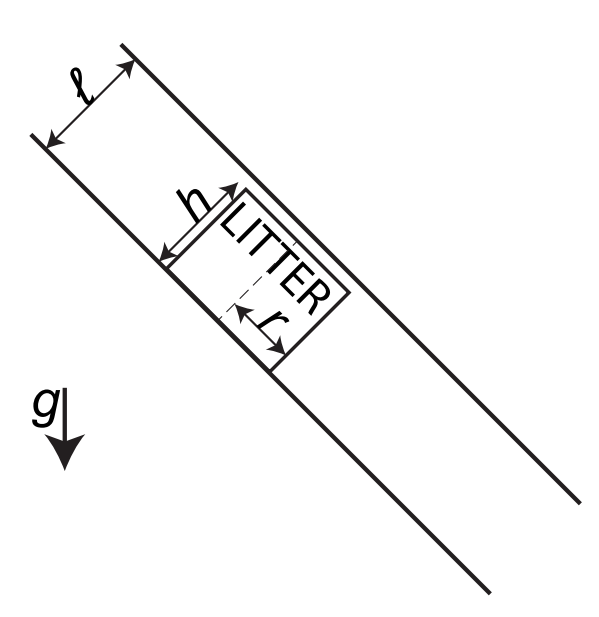
\includegraphics[width=0.5\linewidth]{2013-v3p-04-yl.PNG}
\end{center}
\fi

\ifHint
Litri ühtlase kiirusega libisemisest järeldub, et kogu potentsiaalse energia muutus teisendub litri soojusenergiaks. 
\fi

\ifSolution
Litri ühtlase kiirusega libisemisest järeldub, et kogu potentsiaalse energia muutus teisendub litri soojusenergiaks. Vertikaalsuunas vahemaa $H$ läbimisel kaotab litter potentsiaalset energiat $Q = mgH$ võrra (kus $m$ on litri mass). Litri temperatuur tõuseb selle käigus
\begin{center}
$\triangle T = \frac{Q}{mc} = \frac{mgH}{mc} = \frac{gH}{c}$
\end{center}
võrra ja mõõtmed suurenevad kuni 
\begin{center}
$l = h(1 + \alpha \triangle T) = h(1 + \frac{\alpha g H}{c})$. 
\end{center}
Valemist saab nüüd avaldada maskimaalse vahemaa vertikaalsuunas, mille litter saab läbida enne kinnijäämist:
\begin{center}
$H = \frac{(\cfrac{l}{h} - 1) \cdot c}{\alpha g}$.
\end{center}
\fi
}